\documentclass{standalone}
\usepackage{tikz}
\begin{document}
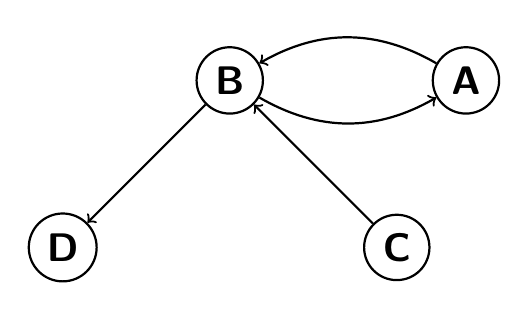
\begin{tikzpicture}[->, node distance=3cm, every loop/.style={},
                    thick,main node/.style={circle,draw,font=\sffamily\Large\bfseries}]

  \node[main node] (1) {A};
  \node[main node] (2) [left of=1] {B};
  \node[main node] (3) [below right of=2] {C};
  \node[main node] (4) [below left of=2] {D};

  \path[every node/.style={font=\sffamily\small}]
    (1) edge [bend right] (2)
    (2) edge [bend right] (1)
    (3) edge [] (2)
    (2) edge [] (4);
\end{tikzpicture}
\end{document}